\documentclass{article}

\usepackage[margin=1in]{geometry}
\usepackage{graphicx} 
\usepackage{gensymb}
\usepackage{amsmath}
\usepackage{multicol}
\usepackage[font=small,labelfont=bf]{caption}

\title{GAN}
\author{Stefan Huber}
\date{December 2022}

\begin{document}
\maketitle
\section{Introduction}
In order to generate the time series of a similar distribution as the original ones, we chose to use a Generative Adversarial Network (GAN). The GAN framework consists of two models, the generator and the discriminator. They learn by “playing” against each other: The generator generates new time series and tries to trick the discriminator into predicting them as real ones, while the predictor learns to distinguish them. Ideally in this process, the predictor learns the distribution of real data and the generator generates series that share exactly this distribution, such that ultimately the discriminator's best choice is to pick at random. \\
Regarding the architecture of generator and discriminator, we draw significant inspiration from Savasta \& Politano (2020). We used a Wasserstein GAN, as this improves training stability and the loss directly correlates with the sample quality, so for more advanced performance evaluation we later can just use the loss function of the generator rather than only see whether the model can fool human eyes.
\section{A first Generator}
A first Generator
The architecture is mainly a combination of linear and convolutional layers and was designed by Fernando (2019), but as Savasta \& Politano (2020) we use RMSprop as optimizer rather than adam. In contrast to them however, we completely remove spectral normalization as it caused model collapse. We use the Xavier uniform initializer to initialize the weights of the model. That way we ensure that the weights of the network are initialized in a way that is well-suited to the activation functions used in the network. This helps to improve the performance of the network by ensuring that the weights are not too small or too large, which can prevent the network from learning effectively. \\
The generator takes a random noise vector of length 50 as input returns a time series vector of length 100. It consists of several layers, each of which applies a different transformation to the input data. The first layer is a linear transformation, which applies a matrix multiplication and a bias term to the input data. This is followed by a Leaky ReLU nonlinearity, which applies a nonlinear function element-wise to the input data. The next layer adds an extra dimension to the input data, which is necessary for the subsequent convolutional layers. \\
Then three 1D convolutional layers follow, which apply a convolution operation to the input data. This operation is a way of extracting local spatial information from the input data. The convolution is followed by an upsampling operation, which increases the size of the data. The upsampling is followed by a dropout layer, which randomly zeroes out some of the input data. This prevents overfitting and increases robustness. Then a fourth convolutional layer follows. \\
Finally a Leaky ReLU applies an element-wise nonlinear function to the input data and the data get squeezed down to a single dimension, and the last layer is a linear transformation, which applies a matrix multiplication and a bias term to the input data.
\begin{center}
    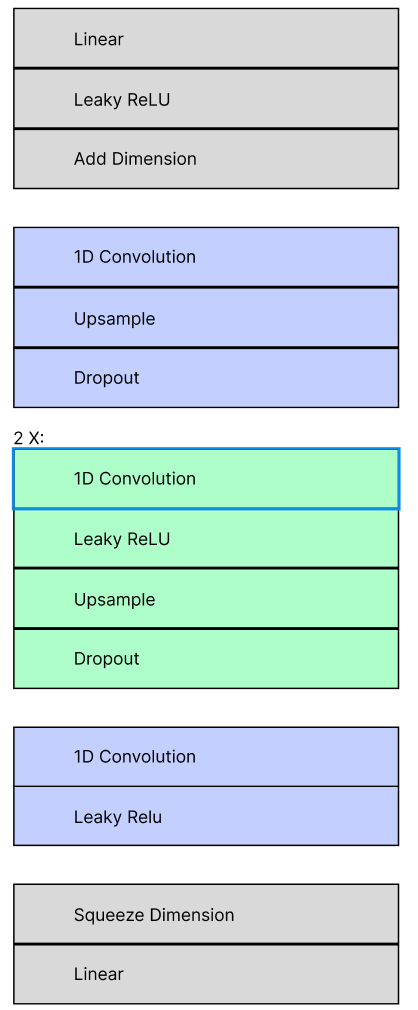
\includegraphics[scale=0.3]{imgs/stefan/generator-graphic-v1.png}
\end{center}

\section{The Discriminator}
The discriminator, also called critic, takes in the generated time series or the original ones as input and returns a single number, indicating whether it predicts the input to be an original or generated time series. With respect to its architecture the critic is very similar to the generator. \\
At first it adds an extra dimension to the input data, which is necessary for the subsequent convolutional layers. Three 1D convolutional layers follow, which apply a convolution operation to the input data to extract local spatial information from the input data. We use spectral normalization to increase training stability as Savasta \& Politano (2020) suggest. Again, the convolution is followed by a Leaky ReLU nonlinearity, which applies a nonlinear function element-wise to the input data. The convolution is also followed by a max pooling operation, which reduces the size of the data by taking the maximum value within a local neighborhood of each element. \\
The next three layers are fully-connected (i.e., linear) layers with varying sizes, which apply a matrix multiplication and a bias term to the input data. These also have Leaky ReLU nonlinearities. The final layer produces a single output value, indicating whether the input data is real or fake.
\begin{center}
    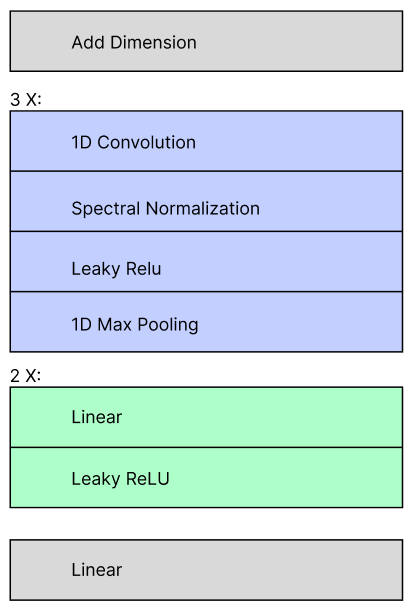
\includegraphics[scale=0.3]{imgs/stefan/discriminator-graphic-v1.png}
\end{center}



    \begin{multicols}{2}
    
    \end{multicols}
\end{document}